% !TeX spellcheck = sv_SE
\section{Inledning}
	
	Detta arbete jämför olika ramverk för uppskalning av agil programutveckling. Dessa beskriver hur man kan utnyttja traditionella agila metoder även i större organisationer och projekt. 
	
	Agila metoder, såsom Scrum, är riktade till grupper på mindre än 10 personer\cite{scrum_guide}, dock finns det projekt för grupper större än det som traditionellt lämpat sig för agil utveckling.
	Behov för metoder att skala upp agil utveckling finns.
	
	I rapporten gjord av Version One \cite{version_one_report} listas det upp ett flertal metoder för uppskalning av agil utveckling. Akademisk forskning om de olika metoderna existerar i stort sett inte alls, vilket gör det utmanande för företag att göra beslut om vilken metod som lämpar sig för deras behov. Även mångfalden av metoder, med mer eller mindre omfattande dokumentation, utgör ett hinder för företag att göra ett beslut om vilken metod de vill implementera. 	
	I detta arbete ämnar man lyfta fram tre metoder för uppskalning av agil utveckling samt analysera och jämföra dom.
	De metoder som beskrivs och jämförs är stödda av tillräcklig egen dokumentation för att klassas som egenstående ramverk, så att arbetet ska kunna tänkas användas som stöd för företag som försöker välja vilket ramverk som passar deras behov.	
	
	Valet av de jämförda ramverken beskrivs noggrannare i stycke 3.
	Syftet är att klargöra ifall det finns klara skilda användningsändamål för ramverken i fråga, samt vilka de största skillnaderna i implementationen är. Som grund för jämförelserna används fallstudier om implementation av ramverken i olika företag. För att jämföra ramverkens egenskaper används teknisk dokumentation som finns tillgänglig på ramverkens webbsidor.
	
	Introduktionen utgör det första kapitlet i arbetet. Det andra kapitlet tar upp bakgrunden, samt går igenom nödvändiga förhandskunskaper. Efter det följer kapitel om syftet samt material och metodik. Fjärde kapitlet presenterar resultaten av materialet. Som sista kapitel sammanfattas arbetet med diskussion om resultaten samt eventuell fortsatt forskning.
	
	
	%meta
	%todo skriv Metatexten EFTER att du har fucking skrivit arbetet
\newpage
\section{Bakgrund}
	
	I detta stycke behandlas den tekniska bakgrunden till arbetet. Central bakgrundskunskap förutsatt av läsaren presenteras här.
	
	\subsection{Agil utveckling}
	
		Agil utveckling är en metod, eller en samling principer, för programutveckling. Principerna bygger på att bryta ner en stor helhet i små mindre självständiga delar, som man sedan utvecklar i skilda etapper, ofta kallade Sprinter.
		Mellan varje sprint finns möjlighet för kunden och utvecklarna att komma med förändringsförslag och kommentera förra sprintens resultat. Varje sprint ska producera en fungerande helhet som läggs till huvudprodukten. Centrala begrepp och principer inom agil programutveckling är transparens, flexibilitet samt inkrementell och iterativ utveckling. Man värdesätter flexibilitet och kommunikation med kunden över en noggrant specificerad process som sedan följs. \cite{agile_manifesto}
		\\
		Några ramverk för agil utveckling är Unified Process (UP), Extreme Programming (XP) och Scrum.
		Scrum hör till de mest kända och allmänt använda ramverket, och som följd har många andra ramverk för både agil utveckling och skalning av detta baserats på Scrum. I detta arbete behandlas till exempel LeSS (Large Scale Scrum), som rakt översatt står för ``Scrum i stor skala''.
		
		Begrepp som förekommer inom Scrum är alltså även återkommande inom agil utveckling och skalning av den.
		
	\subsection{Scrum i korthet}	
		
		Centrala roller i Scrum är produktägare, scrum-mästare och scrum-team. Dessa samverkar genom sprint-planering, dagliga scrum-möten och post-sprint återblick. De upprätthåller bland annat orderstocken.
		
		\textbf{Backlogg} \\
		En lista på delmoment av slutprodukten som ännu ska implementeras. Upprätthålls i huvudsak av produktägaren. \\	
		
		\textbf{Scrum-team} \\
		Består av en grupp på optimalt tre till nio personer. Utvecklar under varje sprint de överenskomna delarna av orderstocken. \\
		
		\textbf{Produktägare} \\
		Upprätthåller orderstocken genom att tydligt presentera och prioritera de olika delarna. \\
		
		\textbf{Scrum-mästare} \\
		Övervakar och ser till att Scrum-principer följs i hela processen. \\
		
		Inför varje sprint hålls en sprint-planering, under vilken de delar ur orderstocken som ska utvecklas under sprinten väljs.
		%todo Skriv om scrum i korthet, men med tyngpunkt på begrepp inom agile.
			
		\cite{scrum_guide}
		

	\subsection{Skalning av agil utveckling}
	%Vad är skalning, hur får mad det att fungera.
		
		Agil utveckling har traditionellt applicerats på låg nivå med små grupper och projekt. Det finns en efterfrågan på agila metoder också när det kommer till större projekt som involverar ett flertal grupper. Som sådan kan inte en agil metod, såsom Scrum, användas eftersom principerna däri bygger på en mindre grupp och kommunikation mellan ett fåtal personer.
		Alla projekt kan inte enkelt brytas ner och fördelas på grupper som faller inom ramen för traditionell agil utveckling, så ett konkret behov för nyare metoder uppstår.
		
		Fokus för uppskalning ligger dock inte på att skapa helt nya metoder och principer, utan snarare på att modifiera tidigare använda metoder så att de lämpar sig i större sammanhang. Agil utveckling i stor skala följer således samma grundprinciper som traditionell agil utveckling. Metoder såsom Scrum implementeras ofta inom ett ramverk för agil uppskalning.

		
	\newpage

\section{Metodik, material och syfte}
	
	
	\subsection{Syfte}
	%TODO: Syftet med arbetet
	
		Syftet med arbetet är att klargöra vilka skillnader det finns mellan olika ramverk för skalning av agil utveckling. Tekniska skillnader i användningen och definitionerna av ramverken pekas ut och analyseras.
		Tyngdpunkten ligger på att redogöra för vilka situationer olika ramverk lämpar sig bättre än andra, och att ställa ramverkens styrkor och svagheter mot varandra. \newline
		
		Forskningsfrågor:
		\begin{enumerate}
			\item Hurudana företag väljer ett visst sorts ramverk
			\item Vilken sorts skillnader finns det i implementationen av de olika ramverken
			\item Vilka tekniska skillnader finns mellan ramverken
		\end{enumerate}
			
	
	\subsection{Avgränsning}
	%TODO: Avgränsa arbetet
	
		Ramverken som jämförs i detta arbete är begränsade till Large Scale Scrum (LeSS), Scaled Agile Framework (SAFe) samt Disciplined Agile Delivery (DAD).
		
		Av dessa tre är LeSS och SAFe mer etablerade och har används i relativt stor utsträckning. DAD är ett nyare ramverk, och har således inte uppnått samma användningsnivå som de andra. DAD fungerar dock som en bra jämförelsepunkt i arbetet i och med att det till skillnad från ett flertal andra metoder styrks av omfattande dokumentation som till sin kvalité är fullt jämförbar med den tillgänglig för Less och SAFe.
		\cite{ask_matrix}
		
		Många metoder för skalning av agil utveckling ligger i gränsområdet mellan att kunna kallas enskilt ramverk eller ej. Den mest populära enligt Agile Scaling Knowledge (ASK) och Version One är Scrum of Scrums \cite{ask_matrix} \cite{version_one_report}. Scrum of Scrums är en enkel förlängning på normal Scrum, där scrum-mästarna för många olika grupper träffas och inom sig har ett eget scrum-möte. Detta är inte tillräckligt för att kunna klassas som egenstående ramverk. Detsamma gäller andra populära metoder såsom Spotifys egna modell, även kallad ''Spotify Model``.
		
	\subsection{Material och metoder}
	%TODO: Beskriv arbtessättet, speciellt för informationssökningens del
		
		Huvudsakligt material för arbetet är fallstudier. Inte innehållet eller utfallen av fallstudierna utan meta-datan som går att få ur de studier som finns tillgängliga, såsom företagets bransch.
				
		Arbetets analys och slutsatser är starkt bundna av tillgången till material och på kvalitén av det tillgängliga materialet. Speciellt fallstudier kan vara vinklade i något visst ramverks fördel, eftersom företag inte vill rapportera dåliga resultat eller misslyckade projekt. Konsulter vill ofta inte heller erkänna att de använt sig av tvivelaktiga metoder.
		Det har liten betydelse då arbetet fokuserar på vilken sorts företag som använde sig av metoden, och inte specifikt hur utfallet blev.
		
		
		Tabell över tillgängligt material för de olika ramverken:

		\begin{center}
		\begin{tabular}{ >{\bfseries}l | r | r | r }
			 	 						& Böcker & Artiklar & Fallstudier 	\\ \hline
			Disciplined Agile Delivery 	& 1 	& 2			& 2 			\\ \hline
			Large Scale Scrum 			& 3 	& >10		& 21 			\\ \hline
			Scaled Agile Framework 		& 4 	& >10		& 27 			\\ 
		\end{tabular}
		\end{center}
		
		Källa: Ramverkens respektive hemsidor\cite{dad_web, less_web, safe_web}, samt sökningar i vetenskapliga databaser(via bl.a. Google Scholar) med ramverken som sökord.
		
		Samtliga ramverk har utförliga hemsidor med mycket allmän information om ramverken.
		
		Ur tabellen ovan går att se en tydlig brist i fallstudier för DAD. Teknisk dokumentation finns till ändamålsenlig grad, men på grund av bristande data om användningsområden förblir analysen till viss mån ytlig för ramverket i fråga.
		Brist på data och fallstudier beror främst på ramverkets begränsade adoption bland större företag.
	
	%Hemsidor:
	%http://www.disciplinedagiledelivery.com/
	%http://scaledagileframework.com/
	%http://less.works/
	
\newpage
\section{Analys, fallstudier och resultat}
	
	
	\subsection{Large-Scale Scrum}
	
	
		Large-Scale Scrum har som grundläggande egenskap Scrum. Scrum-grupper håller egna interna scrum-möten med scrum-mästare, och upprätthåller egna sprint-backloggar. Ovanpå den traditionella Scrum-metodiken existerar produktöversträckande backloggar och sprint-uppföljning.
		
		
		\begin{center}	
			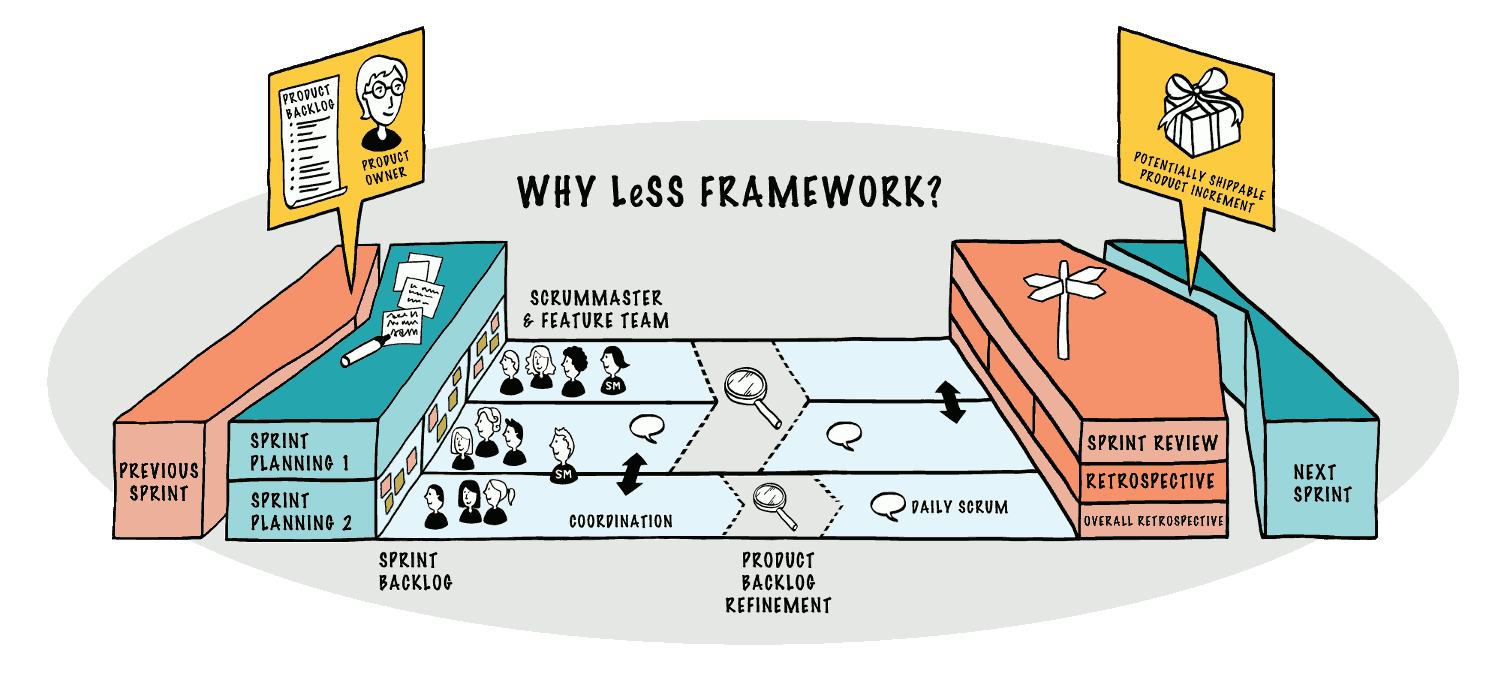
\includegraphics{Material/less_framework.png}
		\end{center}
		%todo Skriv mera om hur LeSS fungerar, knyt till scrum terminologi -> http://less.works/less/framework/index.html
	
		Några grundläggande LeSS principer är: \cite{less_principles}
	
		\begin{itemize}
			\setlength{\itemsep}{1pt}
			\item LeSS är Scrum - använd Scrum-principer oförändrat i ett större sammanhang			
			\item Transparens
			\item ''\textbf{More} with \textbf{LeSS}'' dvs. \textbf{Mera} med \textbf{mindre}
				\begin{itemize}
					\item \textbf{Mer} inlärning med \textbf{mindre} definierade processer
					\item \textbf{Mer} värde med \textbf{mindre} omkostnader
					\item \textbf{Mer} ägarskap och syfte med \textbf{mindre} huvudroller och specialgrupper
				\end{itemize}
			\item Kundcentrerat
			\item Systemtänkande
		\end{itemize}
			
	\subsection{Scaled Agile Framework}
		
		%todo SAFe pls, make it happen
		
		\begin{center}
			\includegraphics[scale=0.2]{Material/SAFeBigPicChart.jpg}
		\end{center}
		Några grundläggande SAFe principer är: \cite{safe_principles}
		\begin{itemize}
			\item Ekonomisk synpunkt
			\item Systemtänkande
			\item Förvänta förändring - bevara möjligheter
			\item Bygg inkrementellt med snabba inlärningsintervall
			\item Basera milstolpar på en objektiv värdering av ett fungerande system
			\item Visualisera och begränsa pågående arbete
		\end{itemize}
			
		
	\subsection{Disciplined Agile}
		
			%todo DAD pls -> http://www.disciplinedagiledelivery.com/introduction-to-dad/
		\begin{center}
			\includegraphics[scale=0.4]{Material/DAD_graphic.jpg}
		\end{center}
		Några grundläggande DAD principer: \cite{dad_principles}
		\begin{itemize}
			\item Tyngdpunkt på tidiga och kontinuerliga leveranser av lösningar
			\item Utnyttja föränderliga krav till att utöka kundens konkurrenskraft
			\item Leverera fungerande del-lösningar med korta tidsintervall
			\item Dagligt samarbete mellan produktens intressenter och utvecklare
			\item Kommunikation som sker ansikte mot ansikte är den mest effektiva till och inom en arbetsgrupp
			\item Fungerande och användbara lösningar är den primära måttstocken för framsteg
		\end{itemize}
			
	
	\subsection{Användningsområden}

		Fallstudier sammanfattar hur implementationen av ramverket i företaget gått och framförallt vilket resultat man uppnått. Det framgår sällan vilken sorts förhandsarbete som gjorts, och vilka kriterier man satt ut innan man valde att använda sig av ett enskilt ramverk.
		
		\subsubsection{Branscher - Data}
			
			För att kunna dra någon form av slutsats gällande vilka orsaker företag har för att välja ramverk har företagen indelats enligt bransch.
					
			Ramverk som favoriserats av en specifik bransch kan antas vara väl mer lämpat för ett dylikt företag än de andra ramverken. DAD har inte tagits i beaktande på grund av bristfällig information och total saknad av fallstudier.
			
			Observera att det inte är ändamålsenligt att jämföra statistiken sinsemellan som sådan, eftersom totala antalet fallstudier är olika. Endast de interna förhållandena mellan branscher inom ett och samma ramverk är intressanta.
				
			Nämnvärt är även att den relativt låga mängden fallstudier gör alla sorters slutsatser dragna på basis av statistiken är svaga.
			
			\title{Large Scale Scrum branscher}
			\begin{center}
				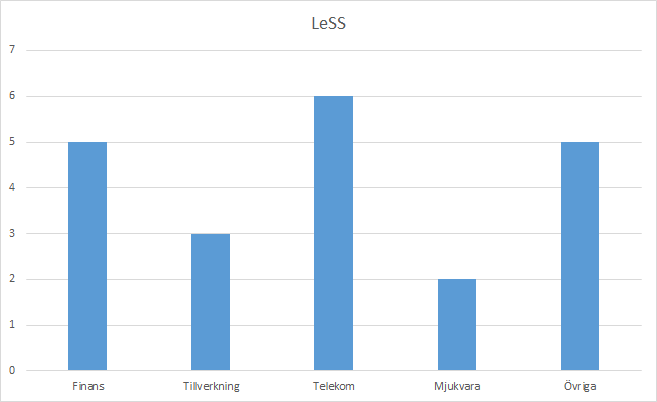
\includegraphics{Grafer/LeSS_brancher.png}
			\end{center}
		
			LeSS har en tyngdpunkt som ligger på finans och telekombranschen. Annars är det mjukvaruföretag och tillverkningsföretag som står ur mängden.\\		
				
				
			\title{Scaled Agile Framework branscher}
			\begin{center}
				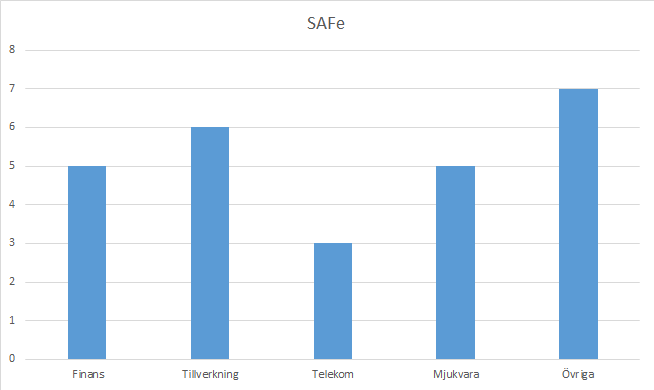
\includegraphics{Grafer/SAFe_brancher.png}
			\end{center}
					
			SAFe har lika som LeSS finansbranschen i toppen, men skiljer sig i och med att både tillverkningsföretag och mjukvaruföretag stiger över telekom.
			
		\subsubsection{Branscher - Slutsatser}
		
			Finansbranschen är återkommande för de båda stora ramverken. Inom finans finns det ovanligt höga krav på säkerhet och kvalité när det kommer till datasystem. Dels på grund av den känsliga datan men främst för att de är en vanlig målgrupp för cyber-kriminalitet. Inom finans finns det heller sällan ekonomiska hinder för projekt av tillräcklig storlek för att behöva tillämpa ett ramverk för uppskalning. 
			
			Institutioner för finans, såsom banker, kan således konstateras vara bland de första som haft både behov och resurser att implementera ramverken.
			
			
			-Telekom vs Tillverkning, förklara skillnaden \\
			-Tillverkning mer strukturerat (tänk löpande band) \\
			-Telekom mer utspritt, dynamiskt. Många olika system som ska fungera. \\
						
		%todo diskutera varför skillnaderna uppstår, dvs telekom vs. tillverkning -> färdig struktur (löpande band etc) vs kaos
	

	\subsection{Popularitet och adoption}
	
		Mängden tillgängligt material ger en riktgivande uppfattning om i vilken utsträckning ramverken används. Mer entydig data finns dock för att stöda uppfattningen och för att ge en tydligare bild.
		
		Enligt en rapport baserad på en enkät gjort av Version one är SAFe betydligt mer utbrett jämfört med LeSS och DAD. \cite{version_one_report} \\	
		
		Observera att man i själva enkäten kunde kryssa flera alternativ, därav en totalprocent på mer än hundra:
		
		\begin{center}
			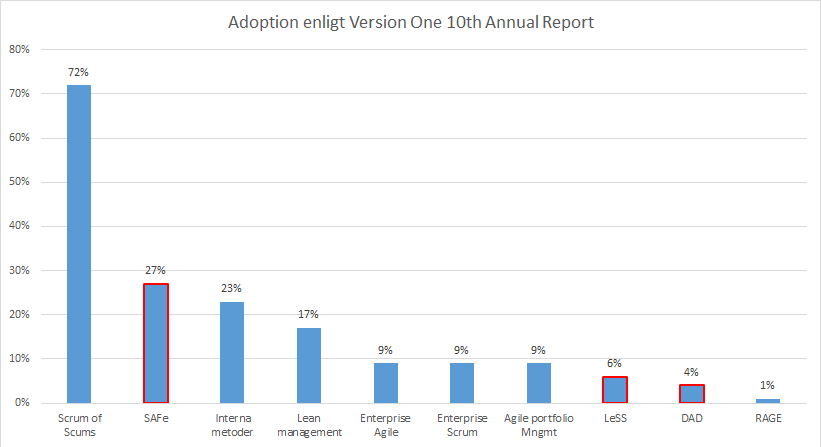
\includegraphics{Grafer/AnnualReport_Adoption.png}
		\end{center}
		\cite{version_one_report}
	
		Den egenskap som korrelerar starkast med ett ramverks eller metods popularitet i ovanstående rapport är kostnad. De mest populära ramverken och metoderna i Version One rapporten har även en implementationskostnad listad som 'låg' i Agile Scaling Knowlegde -matrisen. \cite{ask_matrix}				
		Såsom det påpekas i kapitlet om Material och Metoder är många av de populära metoderna inte klassifierbara som ramverk. 
		
		
		Resultatet från enkäten öppnar inte direkt huruvida ramverken är populära jämfört med varandra, förutom att SAfE är i en klass för sig. Sökmotorn Google ger statistik på popularitet av olika över tiden. I egenskap av världens mest populära sökmotor ger denna statistik en god uppfattning om huruvida ett ramverk är allmänt känt och använt eller ej. 
		
		Då alla tre ramverks sökningar sätts emot varandra kan det igen konstateras att det SAFe är klart mer eftersökt. Ur samma data syns DAD och LeSS som lika eftersökta.
		
		Y-axeln är ett automatiskt genererat jämförelsetal direkt korrelerande med antal sökningar per tidsenhet.
		\begin{center}
			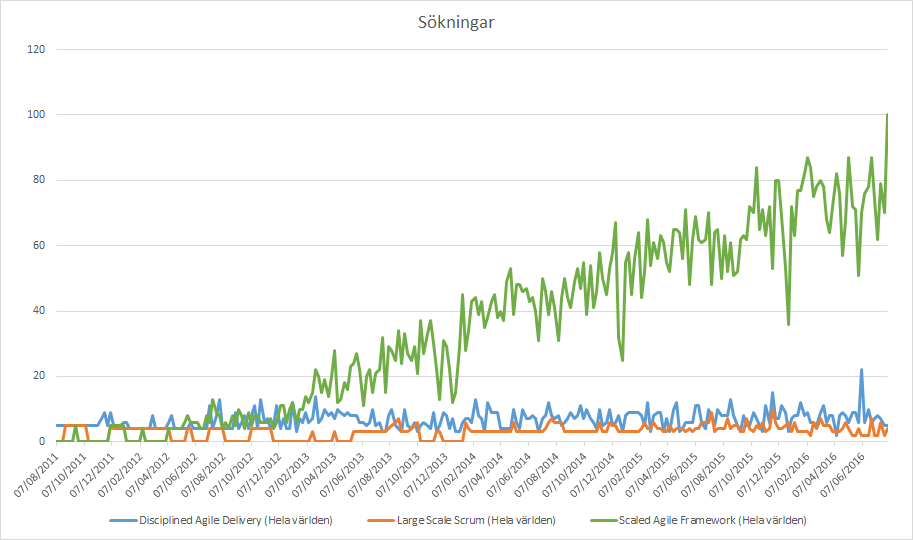
\includegraphics{Grafer/Google_sokningar.png}
		\end{center}
		\cite{google_stats}
	
	
		Genom att utesluta SAFe får man ett noggrannare resultat för LeSS och DAD, vilket är mer ändamålsenligt. DAD genomgår en positivare trend, och är i allmänhet mera eftersökt än LeSS. Detta är motstridigt mot det resultat som rapporterades i Version One rapporten. Detta kan tyda på ett mer utvidgat intresse för DAD i framtiden, då trenden för dess popularitet är klart positiv jämfört med LeSS.
	
		Y-axeln är igen ett jämförelsetal som endast är menat för intern jämförelse inom denna graf.
		\begin{center}
			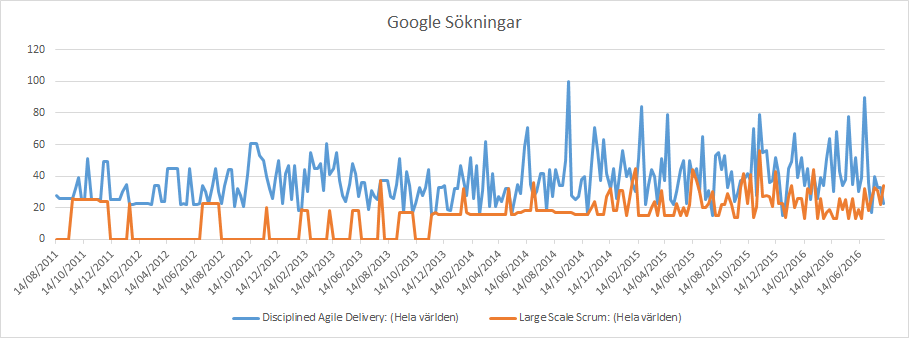
\includegraphics{Grafer/Google_sokningar_dad_less.png}
		\end{center}
		\cite{google_stats_dad_less}
		
		
	\subsection{Jämförelse}
		Ur ASK-matrisen:
		-Kostnader \\
		-Tillgänglig certifikation och skolning
			
				
\section{Diskussion och fortsatt forskning}
	